\documentclass[12pt, twoside, hidelinks, a4paper]{article}

\usepackage[]{geometry}
\geometry{inner=30mm, outer=20mm, top=23mm, bottom=23mm}

\usepackage{mystyle}
\pagestyle{headings}

\usepackage{fancyhdr}
\fancyhf{}
\pagestyle{fancy}
\renewcommand{\headrulewidth}{0pt}
% numery stron: lewa do lewego, prawa do prawego
\fancyfoot[LE,RO]{\thepage}

\fancypagestyle{plain}
{
   \fancyhf{}
\renewcommand{\headrulewidth}{0pt}
% numery stron: lewa do lewego, prawa do prawego
\fancyfoot[LE,RO]{\thepage}
}

\usepackage{pdfpages}
\usepackage{amsfonts}
%\renewcommand{\familydefault}{\sfdefault}
\setlength\parindent{1cm}

\usepackage{indentfirst}
\usepackage[affil-it]{authblk}
\usepackage{smartdiagram}
\usepackage{metalogo}
\usepackage{moreverb}

\let\lll\undefined
\usepackage{amssymb}

\begin{document}
    \setstretch{1.15}
 	\pagenumbering{arabic}

\author{Marcin Waszak}
\title{OWD -- sprawozdanie z projektu}
\date{5 grudnia 2018}
\affil{Wydział Elektroniki i Technik Informacyjnych, Politechnika Warszawska}


\maketitle

\begin{abstract}
Celem projektu jest optymalizacja pracy elektrowni pod względem kosztów jak i możliwości zaspokojenia wzrostu zapotrzebowań na energię ponad normę. Ponadto zostaną porównane techniki optymalizacji wielokryterialnej przy użyciu skalaryzacji \textit{Metodą Ważenia Ocen} (MWO) oraz \textit{Przedziałową Metodą Punktu Odniesienia} (PMPO).
\end{abstract}

\section{Zadanie}
Kod zadania: \textbf{OWD AK5}

Prowadzący projekt: dr inż. Adam Krzemienowski

\section{Analityczne sformułowanie problemu}
$P$ - uporządkowany zbiór okresów,

$T$ - uporządkowany zbiór typów generatorów (T1, T2, T3),

$I$ - uporządkowany zbiór generatorów danego typu,

Przyjmijmy: $p \in P$, $t \in T, i \in I[t]$

\subsection{Parametry}
\begin{itemize}
\item Zapotrzebowanie na moc w danym okresie [MW]

$period\_demand \{P\}$
\item Długości okresów [h]

$period\_length \{P\}$
\item Ilości generatorów [szt]

$available\_generators \{T\}$
\item Obciążenie minimalne generatora [MW]

$power\_min \{T\}$
\item Obciążenie maksymalne generatora [MW]

$power\_max \{T\}$ 
\item Koszt przy minimalnym obciążeniu [PLN/h]

$cost\_min \{T\}$ 
\item Koszt energii powyżej minimalnego obciążenia [PLN/MWh]

$cost\_linear \{T\}$ 
\item Koszt uruchomienia [PLN]

$cost\_start \{T\}$
\item Całkowita wymagana energia w ciągu dnia [MWh]

$demand\_total = \sum_{p}^{p \in P} period\_demand[p] * period\_length[p]$
\end{itemize}

\subsection{Zmienne}
\begin{itemize}

%\item $\forall p \forall t \forall i : active{P,T,I} binary$
\item Flaga binarna informująca, czy zadany generator pracuje w danym okresie

$active\{P,T,I\} \; binary$
\item Moc danego generatora w danym okresie [MW]

$power\{P,T,I\}$
\item Faktyczna moc wszystkich generatorów w danym okresie

$period\_power \; \{p \in P\} = \sum_{t}^{t \in T} \sum_{i}^{i \in I[t]} \; power[p,t,i];$
\item Faktyczna wyprodukowana energia w ciągu dnia [MWh]

$production\_total = \sum_{p}^{p \in P} \; period\_power[p] * period\_length[p]$
\item 

$demand\_increase = \frac{production\_total}{demand\_total}$
\item Flaga zmiany stanu generatora wraz z początkiem danego okresu

(-1 = wyłączono, 0 = bez zmian, 1 = włączono)

$toggled \{p \in P, t \in T, i \in I[t] \} = active[p,t,i] - active[((p+3) mod |P|)+1,t,i]$

Warto wspomnieć, że dzięki użyciu modulo mamy ,,sklejony'' ostatni okres z pierwszym okresem. Z końcem dnia cykl zapotrzebowań się powtarza i ten fakt nasz model uwzględnia.
\item Flaga włączenia generatora z początkiem danego okresu

$started \{p \in P, t \in T, i \in I[t] \} = \frac{toggled[p,t,i]^2 + toggled[p,t,i]}{2}$
\item Koszt włączenia generatora w okresie (0 jeśli nie został włączony) [PLN]

$cost\_launch \{p \in P, t \in T, i \in I[t] \} = cost\_start[t] * started[p,t,i]$
\item Koszt pracy generatora po włączeniu [PLN/h]

$cost\_usage \{p \in P, t \in T, i \in I[t] \} = cost\_min[t] + cost\_linear[t] * (power[p,t,i] - power\_min[t])$
\item Dzienny całkowity koszt pracy elektrowni [PLN]

$cost\_total = \sum_{p}^{p \in P} \; \sum_{t}^{t \in T} \; \sum_{i}^{i \in I[t]} \; (period\_length[p] * cost\_usage[p,t,i] + cost\_launch[p,t,i])$
\end{itemize}


\subsection{Ograniczenia}
\begin{itemize}
%st1
\item Ograniczenie minimalnej mocy generatora. Zmienna binarna wyłącza te ograniczenie, kiedy dany generator nie pracuje

$\forall p \in P \; \forall t \in T \; \forall i \in I[t] \; : power[p,t,i] 
\geqslant power\_min[t] * active[p,t,i]$
%st2
\item Ograniczenie mocy maksymalnej generatora

$\forall p \in P \; \forall t \in T \; \forall i \in I[t] \; : power[p,t,i] \leqslant power\_max[t] * active[p,t,i]$
%st3
\item Każdemu włączonemu generatorowi T1 musi odpowiadać włączony generator T2 lub T3

$sum\_generators \{ p \in P, t \in T \} = \sum_{i}^{i \in I[t]} active[p,t,i]$

$\forall p \in P : sum\_generators[p,T1] \leqslant sum\_generators[p,T2] + sum\_generators[p,T3]$
%st4
\item Faktyczna dostarczana moc w ciągu okresu sprostać zapotrzebowaniom

$\forall p \in P : period_power[p] \geqslant period\_demand[p]$
\end{itemize}

\subsection{Funkcje celu}
\subsubsection{Funkcja celu dla minimalizacji kosztu}
Zapis minimalizacji kosztu jest trywialny:
$$min \: \: \leftarrow cost\_total$$

\subsubsection{Funkcja celu metody ważenia ocen}
Załóżmy, że znamy wartość wagi $weight$, to wtedy funkcja celu wygląda następująco:
$$max \: \: \leftarrow weight*demand\_increase - cost\_total$$
Należy zwrócić uwagę, że $cost\_total$ jest poprzedzone minusem, ponieważ kanonicznie metoda ważenia ocen jest problemem maksymalizacji. My natomiast koszt całkowity chcemy minimalizować. Ponadto zrezygnowano z normalizacji wag, ponieważ w tym wypadku wygodniej dopasować proporcję ważności kryteriów sterując jednym parametrem.

\subsubsection{Funkcja celu dla przedziałowej metody punktu odniesienia}
Załóżmy, że znamy wartości parametrów $\epsilon$, $\gamma$, $\beta$, $a_1$, $r_1$, $a_2$, $r_2$. Wprowadźmy zmienne pomocnicze $v$, $z_1$, $z_2$. Ostatecznie przedziałowa metoda punktu odniesienia może być w zaimplementowana formułując następujące ograniczenia:
\begin{itemize}
\item $v \leqslant z_1$
\item $v \leqslant z_2$
\item $z_1 \leqslant \gamma \; \frac{cost\_total - r_1}{a_1 - r_1}$
\item $z_1 \leqslant \frac{cost\_total - r_1}{a_1 - r_1}$
\item $z_1 \leqslant \beta \; \frac{cost\_total - a_1}{a_1 - r_1} + 1$
\item $z_2 \leqslant \gamma \; \frac{demand\_increase - r_2}{a_2 - r_2}$
\item $z_2 \leqslant \frac{demand\_increase - r_2}{a_2 - r_2}$
\item $z_2 \leqslant \beta \; \frac{demand\_increase - a_2}{a_2 - r_2} + 1$
\end{itemize}
Wtedy funkcja celu ma następującą postać:
$$max \: \: \leftarrow v + \epsilon * (z_1 + z_2)$$

\section{Implementacja}
Powyższy model matematyczny został zaimplementowany w języku AMPL. Jako solver został wybrany CPLEX, ponieważ obsługuje on zmienne dyskretne, w szczególności zmienne binarne.

Implementacja składa się z następujących plików:
\begin{itemize}
\item \textbf{\texttt{owd.mod}} - opis modelu,
\item \textbf{\texttt{owd.dat}} - dane modelu,
\item \textbf{\texttt{owd\_minimize\_cost.run}} - wykonanie minimalizacji kosztu,
\item \textbf{\texttt{owd\_weighted\_objectives.run}} - wykonanie metody ważenia ocen,
\item \textbf{\texttt{owd\_interval\_rpm.run}} - wykonanie przedziałowej metody puntu odniesienia.
\end{itemize}

\subsection{Testowanie poprawności modelu}
Rozwój modelu następował małymi częściami, które były na bieżąco sprawdzane. Po dodaniu każdego ograniczenia weryfikowano manualnie wartości zmiennych decyzyjnych po wykonaniu symulacji. Po ukończeniu modelu przy okazji sporządzania tejże dokumentacji po raz kolejny sprawdzano integralność modelu. Na tym etapie udało się znaleźć drobny błąd, który powodował błędne naliczanie całkowitej wyprodukowanej energii. Zmieniało to rozwiązania funkcji celów używających zmiennej \textbf{production\_total}, czyli w metodzie ważenia ocen oraz przedziałowej metodzie punktu odniesienia. Błąd został usunięty.

\section{Wyniki symulacji}
W tym rozdziale omówimy rezultaty otrzymane z optymalizacji każdej funkcji celu z osobna.

\subsection{Symulacja dla minimalizacji kosztów} \label{sec:cost_min}
Wyznaczanie rozwiązania zajęło 455 iteracji algorytmu simplex. Jest to zatem mało złożone zadanie optymalizacji.

Minimalny koszt: \textbf{819900 PLN}

Wyprodukowana energia w ciągu doby: \textbf{612000 MWh}

A tak prezentują się szczegółowe dane dotyczące mocy każdego generatorów w danym okresie:

\begin{boxedverbatim}
power [*,T1,*] (tr)
:    1    2      3      4      5      :=
1    0   2000    850   2000   2000
2    0   2000   2000   2000      0
3    0    850   1250   1000      0
4    0      0      0   2000      0
5    0      0      0   2000   2000
6    0      0      0   2000   2000
7    0   2000    850   2000      0
8    0      0      0      0      0
9    0      0      0   2000    950
10   0   2000    850   2000    850
11   0   2000    850   2000    850
12   0   1650    850   2000    850

 [*,T2,*] (tr)
:     1      2      3      4      5      :=
1    1250   1750   1750   1750   1750
2    1250   1750   1750   1750   1750
3    1250   1750   1750   1750   1750
4    1750   1750   1750   1750   1750
5    1250   1750   1750   1750   1750
6    1750   1750   1750   1750   1750
7    1250   1750   1750   1750   1750
8    1750   1750   1750   1750   1750
9    1750   1750   1750   1750   1750
10   1750   1750   1750   1750   1750

 [*,T3,*] (tr)
:   1   2   3    4     5    :=
1   0   0   0      0   0
2   0   0   0      0   0
3   0   0   0   1500   0
4   0   0   0      0   0
5   0   0   0      0   0
\end{boxedverbatim}

Wyniki zostały pogrupowane według typów generatorów. Rzędy opisują konkretne generatory, natomiast kolumny opisują okresy. Możemy łatwo posumować kolumny, w rezultacie możemy zobaczyć, że nasze rozwiązanie faktycznie prezentuje wymagane moce w kolejnych okresach opisane w zadaniu.

Otrzymane rozwiązanie jest o tyle ciekawe, że okazuje się, iż nie opłaca się wyłączać żadnego z generatorów typu \textbf{T2}. Każdy z generatorów tego typu prawie zawsze pracuje z maksymalną dopuszczalną dla niego mocą (wyjątkiem jest okres 1. kiedy obciążenie sieci energetycznej jest na wyjątkowo małym poziomie). Wniosek jest taki, że czynnikiem przeważającym wybór tego typu generatora jest jego niski koszt powyżej minimalnego obciążenia. Drugim najczęściej wybieranym jest generator typu \textbf{T1}. Najmniej opłacalnym jest natomiast \textbf{T3}.

\subsection{Symulacja dla metody ważenia ocen} \label{sec:weight}
W tej metodzie w zależności przy pomocy parametru \textbf{weight} możemy ustawić, która ocena ma dla nas większe znaczenie. Kiedy wartość parametru jest niska to większe znaczenie ma dla nas minimalizacja kosztu. Kiedy natomiast waga rośnie, to ważniejsze z punktu widzenia optymalizacji jest maksymalizacja większego zapotrzebowania. Jako, iż ustawienie parametru nie jest oczywiste postanowiono dokonać przemiatania wartości \textbf{weight} od 100000 do 2000000 ze skokiem o 10000.

Dokonano symulacji dla wyżej wymienionych wartości. Złożoność wynosiła od 60 do 600 iteracji simplex (średnio dla 200 iteracji dla wartości \textbf{weight}, które nie były skrajne).

Pozwoliło nam to wykreślić zależność w przestrzeni ocen (względny wzrost produkcji - koszt). Rezultat prezentuje rysunek \ref{fig:plot}.

\begin{figure}[H]
\centering
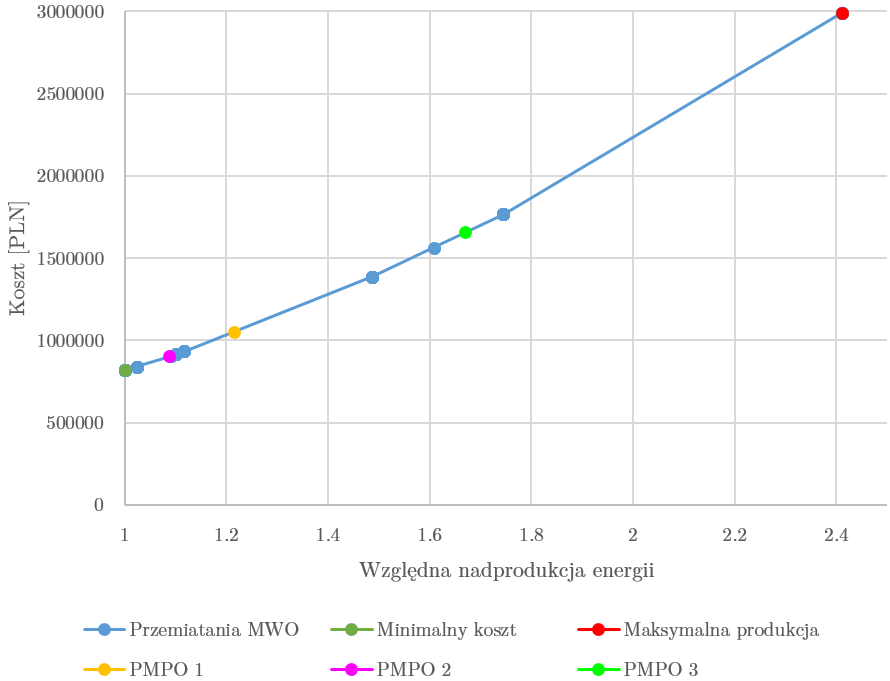
\includegraphics[scale=0.4]{plot_new.png}
\caption{Przestrzeń rozwiązań efektywnych w przestrzeni względnej produkcji i kosztu}
\label{fig:plot}
\end{figure}

Kolor niebieski to wykres osiągniętego kosztu od względnej nadprodukcji energii. Ponadto widzimy, że nasza symulacja dotarła do skrajnych ocen, tj. osiągnęliśmy minimalny koszt prezentowany w podpunkcie \ref{sec:cost_min} oraz przypadek maksymalnej produkcji energii (wszystkie generatory pracujące z maksymalną mocą przez wszystkie okresy doby). Wartości skrajne są oznaczone kolorem ciemnozielonym i czerwonym. Pozostałe zaznaczone punkty, dotyczą kolejnego podrozdziału \ref{sec:pmpo}.

\subsection{Symulacja dla przedziałowej metody punktu odniesienia} \label{sec:pmpo}
Metoda użyta w tym podpunkcie jest bardziej zaawansowaną metodą skalaryzacji wielokryterialnej. Jest to metoda interaktywna, w której ustawiamy parametry aspiracji i rezerwacji (wartości pożądanej i wymaganej). Metoda ta pomaga decydentowi podjąć wybór, dzięki tym intuicyjnym punktom odniesienia.

Dokonano symulacji przy użyciu tej metody. W pierwszej kolejności rzuca się w oczy drastyczny wzrost złożoności obliczeniowej problemu. W zależności od parametrów $\epsilon$, $\gamma$, $\beta$, $a_1$, $r_1$, $a_2$, $r_2$ złożoność zmienia się od dziesiątek tysięcy do dziesiątek milionów iteracji. Przykładowe wartości ocen i złożoności w zależności od parametrów PMPO:

\begin{table}[H]
\begin{tabular}{llllllllll}
$\epsilon$ & $\gamma$ & $\beta$ & $a_1$ & $r_1$ & $a_2$ & $r_2$ & \textbf{produkcja} & \textbf{koszt [PLN]} & $l. iteracji$ \\ \hline
0.001                            & 1000                           & 0.001                         & 880000        & 1400000       & 1.3           & 1.05          & \textbf{1.21628}            & \textbf{1054130}        & \texttt{156466}               \\
0.001                            & 100                            & 0.01                          & 819900        & 900000        & 1.5           & 1.1           & \textbf{1.08793}            & \textbf{902417}         & \texttt{17282212}             \\
0.001                            & 1000                           & 0.001                         & 1000000       & 1400000       & 2             & 1.8           & \textbf{1.67032}            & \textbf{1659370}        & \texttt{2295970}             
\end{tabular}
\end{table}

Wszystkie trzy przypadki zebrane w tabeli umieszczono na rysunku \ref{fig:plot} jako punkty \textbf{PMPO 1}, \textbf{PMPO 2}, \textbf{PMPO 3} (odpowiednio kolory: żółty, różowy, jaskrawozielony). Co ciekawe, wszystkie te rozwiązania efektywne pokrywają się z tymi, do których wcześniej dotarliśmy metodą ważenia ocen co opisano w podrozdziale \ref{sec:weight}. Co ciekawe, PMPO teoretycznie pozwala dotrzeć do punktów nieosiągalnych MWO. Jednakże w naszym przypadku nie zaobserwowałem tego pomimo prób.

\section{Podsumowanie i wnioski}
\begin{enumerate}
\item Cena energii jest w przybliżeniu liniowa w zależności od ilości jaka została wyprodukowana. Trzeba przyznać, że dla wyższych ilości energii wykres zaczyna być bardziej stromy. Wynika to z tego, że jesteśmy zmuszeni korzystać z coraz to droższych generatorów.
\item Generatory typu \textbf{T2} są najtańsze w użytkowaniu, w związku z tym nie opłaca ich się nawet wyłączać.
\item Na wykresie \ref{fig:plot}. nie widać skoków wynikających z włączeń generatorów, ponieważ koszty uruchomienia są znacznie niższe od kosztów pracy.
\item MWO nie wprowadza dodatkowej złożoności do modelu, dzięki czemu możemy z łatwością przeprowadzić przemiatanie wszystkich wartości wagi. Z kolei PMPO wprowadza zauważalne znaczne narzuty złożoności.
\item W ogólności PMPO pozwala nam dotrzeć do rozwiązań efektywnych nieosiągalnych przez MWO. Jednakże w naszym przypadku się to nie udało.
\item W przypadku naszego problemu, który jest dwukryterialny (wzrost energii, koszt) łatwiejsze jest użycie MWO, ponieważ możemy dokonać łatwego przemiatania zmieniając jeden parametr. Jednakże w ogólności w problemach wielowymiarowych bardziej intuicyjne byłoby użycie PMPO. Wynika to stąd, że w przypadku wielu kryteriów łatwiej sterować symulacją ustawiając kolejne poziomy aspiracji i rezerwacji dla każdego kryterium.
\item Na pytanie postawione w zadaniu o wyznaczenie minimalnego kosztu przy możliwości obsługi jak największego względnego wzrostu zapotrzebowań, odpowiedź jest następująca. Nie da się znaleźć jednoznacznego rozwiązania. Bowiem wraz ze wzrostem produkcji koszt będzie zawsze rosnąć. Trzeba więc zdecydować się na pewien kompromis. Po analizie rysunku \ref{fig:plot}. można powiedzieć, że najbardziej warto to zrobić przy mniejszym stopniu nadprodukcji energii ponad normę, gdzie wykres jest najmniej stromy. Może być to zatem okolica punktu \textbf{PMPO 2}, czyli nadprodukcja rzędu ok. 8\% - 10\%. Warto wspomnieć, że tak naprawdę my jako decydenci w elektrowni mamy ograniczone możliwości sterowania produkcją energii. Z praw fizyki wynika, że generatory mają taką moc, jakie panuje w danym momencie obciążenie linii zasilających przez wszystkie odbiorniki w sieci energetycznej. Tak więc nie mamy na to dużego wpływu. Należy jedynie uważać, aby generatory nie przekraczały swoich mocy znamionowych. Można rozważać sztuczną nadprodukcję energii, aby magazynować ją np. w akumulatorach, ale z powodu małej sprawności jest to bez sensu i lepiej przesyłać energię na bieżąco. Wyjątkiem są np. elektrownie wiatrowe lub słoneczne, gdzie musimy magazynować energię, ponieważ zjawiska pogodowe nie zawsze są w stanie dostarczać nam jej dostatecznie dużo, kiedy akurat jej potrzebujemy.
\end{enumerate}

%\printbibliography

\end{document}
